\documentclass[1p]{elsarticle_modified}
%\bibliographystyle{elsarticle-num}

%\usepackage[colorlinks]{hyperref}
%\usepackage{abbrmath_seonhwa} %\Abb, \Ascr, \Acal ,\Abf, \Afrak
\usepackage{amsfonts}
\usepackage{amssymb}
\usepackage{amsmath}
\usepackage{amsthm}
\usepackage{scalefnt}
\usepackage{amsbsy}
\usepackage{kotex}
\usepackage{caption}
\usepackage{subfig}
\usepackage{color}
\usepackage{graphicx}
\usepackage{xcolor} %% white, black, red, green, blue, cyan, magenta, yellow
\usepackage{float}
\usepackage{setspace}
\usepackage{hyperref}

\usepackage{tikz}
\usetikzlibrary{arrows}

\usepackage{multirow}
\usepackage{array} % fixed length table
\usepackage{hhline}

%%%%%%%%%%%%%%%%%%%%%
\makeatletter
\renewcommand*\env@matrix[1][\arraystretch]{%
	\edef\arraystretch{#1}%
	\hskip -\arraycolsep
	\let\@ifnextchar\new@ifnextchar
	\array{*\c@MaxMatrixCols c}}
\makeatother %https://tex.stackexchange.com/questions/14071/how-can-i-increase-the-line-spacing-in-a-matrix
%%%%%%%%%%%%%%%

\usepackage[normalem]{ulem}

\newcommand{\msout}[1]{\ifmmode\text{\sout{\ensuremath{#1}}}\else\sout{#1}\fi}
%SOURCE: \msout is \stkout macro in https://tex.stackexchange.com/questions/20609/strikeout-in-math-mode

\newcommand{\cancel}[1]{
	\ifmmode
	{\color{red}\msout{#1}}
	\else
	{\color{red}\sout{#1}}
	\fi
}

\newcommand{\add}[1]{
	{\color{blue}\uwave{#1}}
}

\newcommand{\replace}[2]{
	\ifmmode
	{\color{red}\msout{#1}}{\color{blue}\uwave{#2}}
	\else
	{\color{red}\sout{#1}}{\color{blue}\uwave{#2}}
	\fi
}

\newcommand{\Sol}{\mathcal{S}} %segment
\newcommand{\D}{D} %diagram
\newcommand{\A}{\mathcal{A}} %arc


%%%%%%%%%%%%%%%%%%%%%%%%%%%%%5 test

\def\sl{\operatorname{\textup{SL}}(2,\Cbb)}
\def\psl{\operatorname{\textup{PSL}}(2,\Cbb)}
\def\quan{\mkern 1mu \triangleright \mkern 1mu}

\theoremstyle{definition}
\newtheorem{thm}{Theorem}[section]
\newtheorem{prop}[thm]{Proposition}
\newtheorem{lem}[thm]{Lemma}
\newtheorem{ques}[thm]{Question}
\newtheorem{cor}[thm]{Corollary}
\newtheorem{defn}[thm]{Definition}
\newtheorem{exam}[thm]{Example}
\newtheorem{rmk}[thm]{Remark}
\newtheorem{alg}[thm]{Algorithm}

\newcommand{\I}{\sqrt{-1}}
\begin{document}

%\begin{frontmatter}
%
%\title{Boundary parabolic representations of knots up to 8 crossings}
%
%%% Group authors per affiliation:
%\author{Yunhi Cho} 
%\address{Department of Mathematics, University of Seoul, Seoul, Korea}
%\ead{yhcho@uos.ac.kr}
%
%
%\author{Seonhwa Kim} %\fnref{s_kim}}
%\address{Center for Geometry and Physics, Institute for Basic Science, Pohang, 37673, Korea}
%\ead{ryeona17@ibs.re.kr}
%
%\author{Hyuk Kim}
%\address{Department of Mathematical Sciences, Seoul National University, Seoul 08826, Korea}
%\ead{hyukkim@snu.ac.kr}
%
%\author{Seokbeom Yoon}
%\address{Department of Mathematical Sciences, Seoul National University, Seoul, 08826,  Korea}
%\ead{sbyoon15@snu.ac.kr}
%
%\begin{abstract}
%We find all boundary parabolic representation of knots up to 8 crossings.
%
%\end{abstract}
%\begin{keyword}
%    \MSC[2010] 57M25 
%\end{keyword}
%
%\end{frontmatter}

%\linenumbers
%\tableofcontents
%
\newcommand\colored[1]{\textcolor{white}{\rule[-0.35ex]{0.8em}{1.4ex}}\kern-0.8em\color{red} #1}%
%\newcommand\colored[1]{\textcolor{white}{ #1}\kern-2.17ex	\textcolor{white}{ #1}\kern-1.81ex	\textcolor{white}{ #1}\kern-2.15ex\color{red}#1	}

{\Large $\underline{12n_{0644}~(K12n_{0644})}$}

\setlength{\tabcolsep}{10pt}
\renewcommand{\arraystretch}{1.6}
\vspace{1cm}\begin{tabular}{m{100pt}>{\centering\arraybackslash}m{274pt}}
\multirow{5}{120pt}{
	\centering
	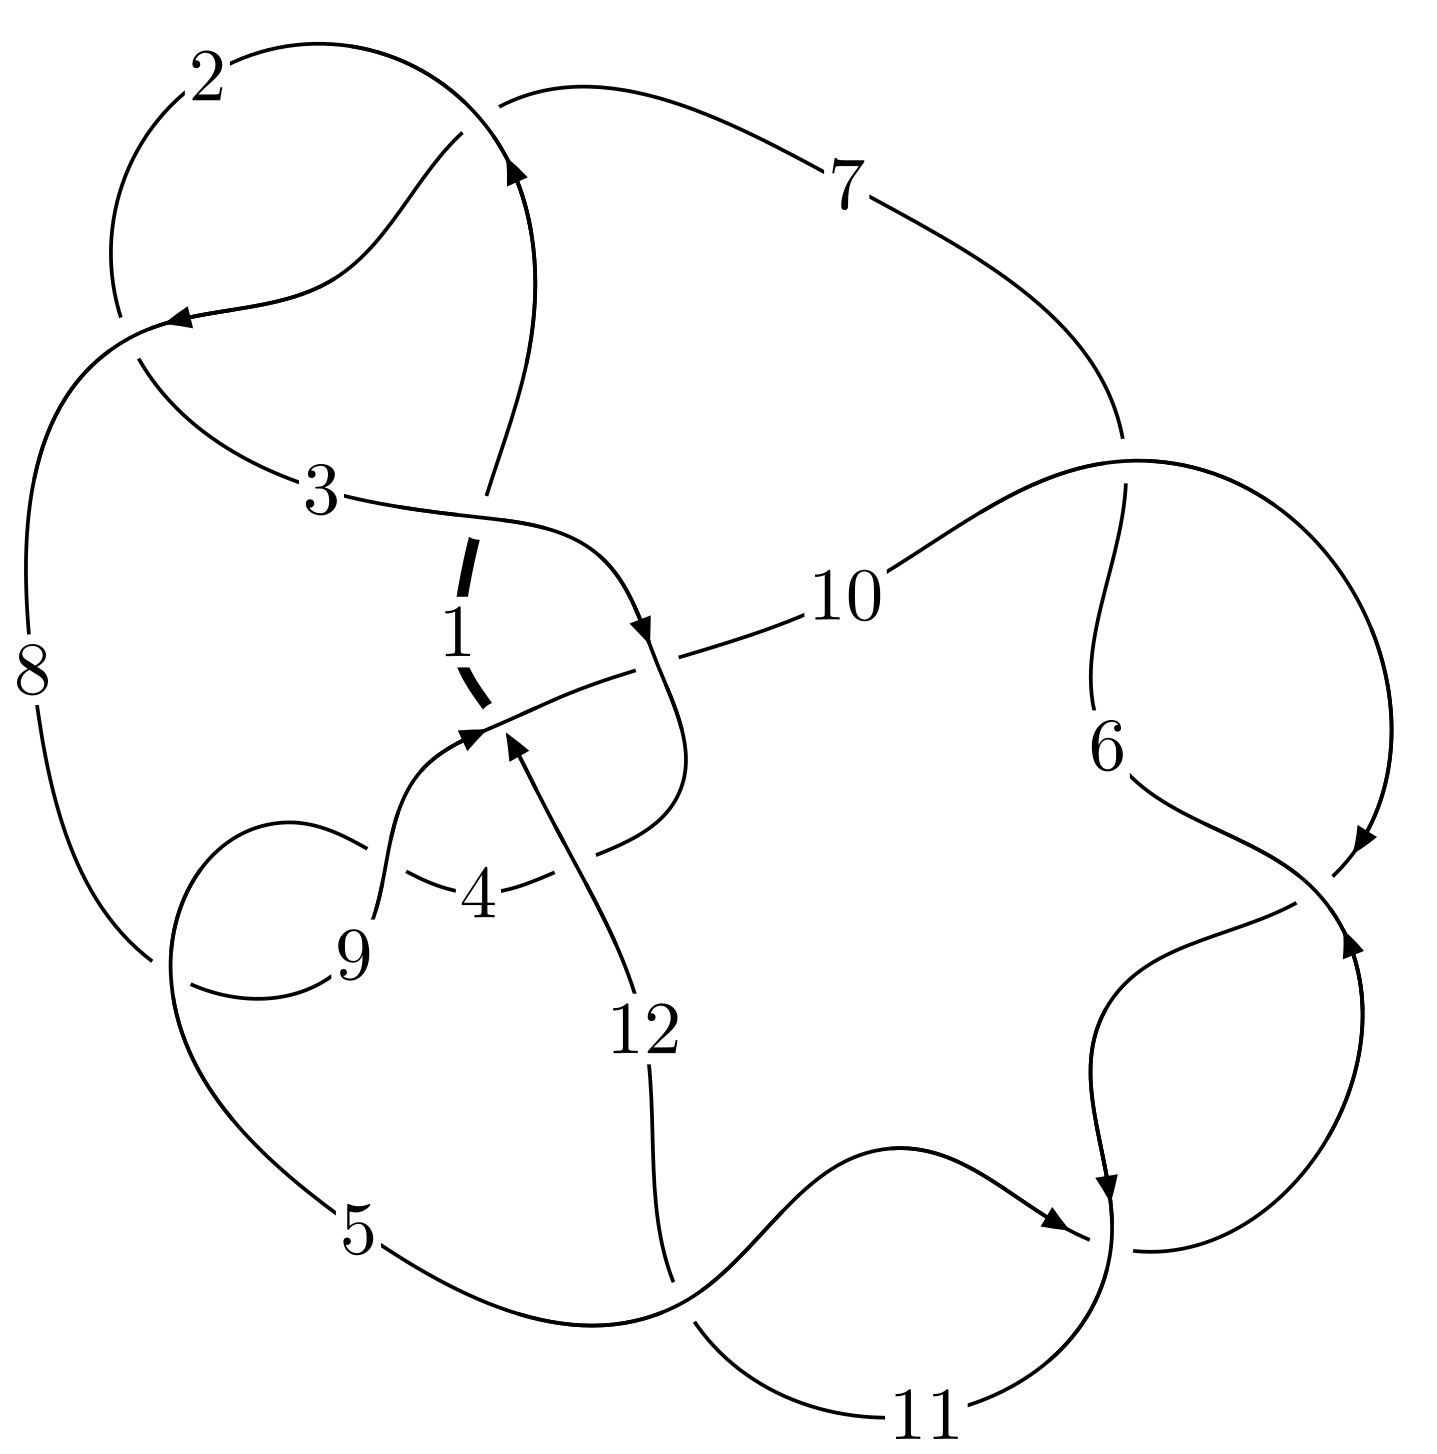
\includegraphics[width=112pt]{../../../GIT/diagram.site/Diagrams/png/2733_12n_0644.png}\\
\ \ \ A knot diagram\footnotemark}&
\allowdisplaybreaks
\textbf{Linearized knot diagam} \\
\cline{2-2}
 &
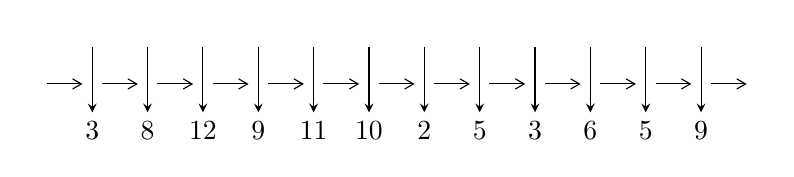
\begin{tikzpicture}[x=20pt, y=17pt]
	% nodes
	\node (C0) at (0, 0) {};
	\node (C1) at (1, 0) {};
	\node (C1U) at (1, +1) {};
	\node (C1D) at (1, -1) {3};

	\node (C2) at (2, 0) {};
	\node (C2U) at (2, +1) {};
	\node (C2D) at (2, -1) {8};

	\node (C3) at (3, 0) {};
	\node (C3U) at (3, +1) {};
	\node (C3D) at (3, -1) {12};

	\node (C4) at (4, 0) {};
	\node (C4U) at (4, +1) {};
	\node (C4D) at (4, -1) {9};

	\node (C5) at (5, 0) {};
	\node (C5U) at (5, +1) {};
	\node (C5D) at (5, -1) {11};

	\node (C6) at (6, 0) {};
	\node (C6U) at (6, +1) {};
	\node (C6D) at (6, -1) {10};

	\node (C7) at (7, 0) {};
	\node (C7U) at (7, +1) {};
	\node (C7D) at (7, -1) {2};

	\node (C8) at (8, 0) {};
	\node (C8U) at (8, +1) {};
	\node (C8D) at (8, -1) {5};

	\node (C9) at (9, 0) {};
	\node (C9U) at (9, +1) {};
	\node (C9D) at (9, -1) {3};

	\node (C10) at (10, 0) {};
	\node (C10U) at (10, +1) {};
	\node (C10D) at (10, -1) {6};

	\node (C11) at (11, 0) {};
	\node (C11U) at (11, +1) {};
	\node (C11D) at (11, -1) {5};

	\node (C12) at (12, 0) {};
	\node (C12U) at (12, +1) {};
	\node (C12D) at (12, -1) {9};
	\node (C13) at (13, 0) {};

	% arrows
	\draw[->,>={angle 60}]
	(C0) edge (C1) (C1) edge (C2) (C2) edge (C3) (C3) edge (C4) (C4) edge (C5) (C5) edge (C6) (C6) edge (C7) (C7) edge (C8) (C8) edge (C9) (C9) edge (C10) (C10) edge (C11) (C11) edge (C12) (C12) edge (C13) ;	\draw[->,>=stealth]
	(C1U) edge (C1D) (C2U) edge (C2D) (C3U) edge (C3D) (C4U) edge (C4D) (C5U) edge (C5D) (C6U) edge (C6D) (C7U) edge (C7D) (C8U) edge (C8D) (C9U) edge (C9D) (C10U) edge (C10D) (C11U) edge (C11D) (C12U) edge (C12D) ;
	\end{tikzpicture} \\
\hhline{~~} \\& 
\textbf{Solving Sequence} \\ \cline{2-2} 
 &
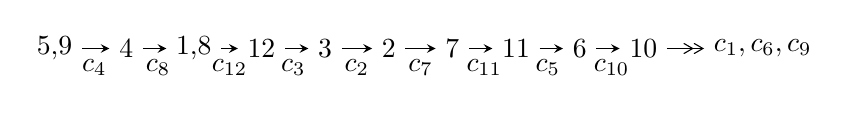
\begin{tikzpicture}[x=23pt, y=7pt]
	% node
	\node (A0) at (-1/8, 0) {5,9};
	\node (A1) at (1, 0) {4};
	\node (A2) at (33/16, 0) {1,8};
	\node (A3) at (25/8, 0) {12};
	\node (A4) at (33/8, 0) {3};
	\node (A5) at (41/8, 0) {2};
	\node (A6) at (49/8, 0) {7};
	\node (A7) at (57/8, 0) {11};
	\node (A8) at (65/8, 0) {6};
	\node (A9) at (73/8, 0) {10};
	\node (C1) at (1/2, -1) {$c_{4}$};
	\node (C2) at (3/2, -1) {$c_{8}$};
	\node (C3) at (21/8, -1) {$c_{12}$};
	\node (C4) at (29/8, -1) {$c_{3}$};
	\node (C5) at (37/8, -1) {$c_{2}$};
	\node (C6) at (45/8, -1) {$c_{7}$};
	\node (C7) at (53/8, -1) {$c_{11}$};
	\node (C8) at (61/8, -1) {$c_{5}$};
	\node (C9) at (69/8, -1) {$c_{10}$};
	\node (A10) at (11, 0) {$c_{1},c_{6},c_{9}$};

	% edge
	\draw[->,>=stealth]	
	(A0) edge (A1) (A1) edge (A2) (A2) edge (A3) (A3) edge (A4) (A4) edge (A5) (A5) edge (A6) (A6) edge (A7) (A7) edge (A8) (A8) edge (A9) ;
	\draw[->>,>={angle 60}]	
	(A9) edge (A10);
\end{tikzpicture} \\ 

\end{tabular} \\

\footnotetext{
The image of knot diagram is generated by the software ``\textbf{Draw programme}" developed by Andrew Bartholomew(\url{http://www.layer8.co.uk/maths/draw/index.htm\#Running-draw}), where we modified some parts for our purpose(\url{https://github.com/CATsTAILs/LinksPainter}).
}\phantom \\ \newline 
\centering \textbf{Ideals for irreducible components\footnotemark of $X_{\text{par}}$} 
 
\begin{align*}
I^u_{1}&=\langle 
-9649326548650 u^{14}+50820393580641 u^{13}+\cdots+871991330612 b+276658983707276,\\
\phantom{I^u_{1}}&\phantom{= \langle  }-98118943388815 u^{14}+517725352137249 u^{13}+\cdots+1743982661224 a+2846447135872992,\\
\phantom{I^u_{1}}&\phantom{= \langle  }u^{15}-5 u^{14}+\cdots-36 u-8\rangle \\
I^u_{2}&=\langle 
37 u^{11}-4 u^{10}-19 u^9-51 u^8-94 u^7+35 u^6+152 u^5-47 u^4+184 u^3-53 u^2+86 b-97 u-25,\\
\phantom{I^u_{2}}&\phantom{= \langle  }11 u^{11}-7 u^{10}- u^9-14 u^8-14 u^7+29 u^6+51 u^5-7 u^4+64 u^3-82 u^2+43 a-30 u-76,\\
\phantom{I^u_{2}}&\phantom{= \langle  }u^{12}+u^{11}+u^{10}-3 u^8-3 u^7- u^6-3 u^5+3 u^4+u^3-1\rangle \\
\\
\end{align*}
\raggedright * 2 irreducible components of $\dim_{\mathbb{C}}=0$, with total 27 representations.\\
\footnotetext{All coefficients of polynomials are rational numbers. But the coefficients are sometimes approximated in decimal forms when there is not enough margin.}
\newpage
\renewcommand{\arraystretch}{1}
\centering \section*{I. $I^u_{1}= \langle -9.65\times10^{12} u^{14}+5.08\times10^{13} u^{13}+\cdots+8.72\times10^{11} b+2.77\times10^{14},\;-9.81\times10^{13} u^{14}+5.18\times10^{14} u^{13}+\cdots+1.74\times10^{12} a+2.85\times10^{15},\;u^{15}-5 u^{14}+\cdots-36 u-8 \rangle$}
\flushleft \textbf{(i) Arc colorings}\\
\begin{tabular}{m{7pt} m{180pt} m{7pt} m{180pt} }
\flushright $a_{5}=$&$\begin{pmatrix}1\\0\end{pmatrix}$ \\
\flushright $a_{9}=$&$\begin{pmatrix}0\\u\end{pmatrix}$ \\
\flushright $a_{4}=$&$\begin{pmatrix}1\\- u^2\end{pmatrix}$ \\
\flushright $a_{1}=$&$\begin{pmatrix}56.2614 u^{14}-296.864 u^{13}+\cdots-1427.56 u-1632.15\\11.0659 u^{14}-58.2808 u^{13}+\cdots-271.998 u-317.273\end{pmatrix}$ \\
\flushright $a_{8}=$&$\begin{pmatrix}u\\u\end{pmatrix}$ \\
\flushright $a_{12}=$&$\begin{pmatrix}56.2614 u^{14}-296.864 u^{13}+\cdots-1427.56 u-1632.15\\6.82466 u^{14}-35.8416 u^{13}+\cdots-162.048 u-192.819\end{pmatrix}$ \\
\flushright $a_{3}=$&$\begin{pmatrix}-64.6576 u^{14}+341.081 u^{13}+\cdots+1634.51 u+1875.21\\-3.15293 u^{14}+16.6942 u^{13}+\cdots+82.5222 u+92.8366\end{pmatrix}$ \\
\flushright $a_{2}=$&$\begin{pmatrix}-59.9171 u^{14}+316.162 u^{13}+\cdots+1519.44 u+1740.30\\1.58748 u^{14}-8.22498 u^{13}+\cdots-32.5463 u-42.0757\end{pmatrix}$ \\
\flushright $a_{7}=$&$\begin{pmatrix}-69.1241 u^{14}+364.539 u^{13}+\cdots+1748.19 u+2001.69\\-2.05249 u^{14}+10.7120 u^{13}+\cdots+51.5981 u+57.9377\end{pmatrix}$ \\
\flushright $a_{11}=$&$\begin{pmatrix}63.0861 u^{14}-332.705 u^{13}+\cdots-1589.61 u-1824.97\\6.82466 u^{14}-35.8416 u^{13}+\cdots-162.048 u-192.819\end{pmatrix}$ \\
\flushright $a_{6}=$&$\begin{pmatrix}31.2918 u^{14}-165.106 u^{13}+\cdots-792.337 u-906.764\\0.796083 u^{14}-4.30252 u^{13}+\cdots-26.8018 u-26.2397\end{pmatrix}$ \\
\flushright $a_{10}=$&$\begin{pmatrix}81.7883 u^{14}-431.479 u^{13}+\cdots-2072.39 u-2372.03\\7.57555 u^{14}-40.0591 u^{13}+\cdots-195.899 u-222.593\end{pmatrix}$\\&\end{tabular}
\flushleft \textbf{(ii) Obstruction class $= -1$}\\~\\
\flushleft \textbf{(iii) Cusp Shapes $= \frac{23777727583517}{217997832653} u^{14}-\frac{125538144456213}{217997832653} u^{13}+\cdots-\frac{605427961030606}{217997832653} u-\frac{696103351358110}{217997832653}$}\\~\\
\newpage\renewcommand{\arraystretch}{1}
\flushleft \textbf{(iv) u-Polynomials at the component}\newline \\
\begin{tabular}{m{50pt}|m{274pt}}
Crossings & \hspace{64pt}u-Polynomials at each crossing \\
\hline $$\begin{aligned}c_{1}\end{aligned}$$&$\begin{aligned}
&u^{15}+23 u^{14}+\cdots+6467 u+961
\end{aligned}$\\
\hline $$\begin{aligned}c_{2},c_{7}\end{aligned}$$&$\begin{aligned}
&u^{15}+u^{14}+\cdots+71 u+31
\end{aligned}$\\
\hline $$\begin{aligned}c_{3}\end{aligned}$$&$\begin{aligned}
&u^{15}-4 u^{14}+\cdots+312 u+49
\end{aligned}$\\
\hline $$\begin{aligned}c_{4},c_{8}\end{aligned}$$&$\begin{aligned}
&u^{15}-5 u^{14}+\cdots-36 u-8
\end{aligned}$\\
\hline $$\begin{aligned}c_{5},c_{6},c_{10}\\c_{11}\end{aligned}$$&$\begin{aligned}
&u^{15}+u^{14}+\cdots-6 u-1
\end{aligned}$\\
\hline $$\begin{aligned}c_{9}\end{aligned}$$&$\begin{aligned}
&u^{15}- u^{14}+\cdots-167 u-151
\end{aligned}$\\
\hline $$\begin{aligned}c_{12}\end{aligned}$$&$\begin{aligned}
&u^{15}+3 u^{14}+\cdots-10 u-4
\end{aligned}$\\
\hline
\end{tabular}\\~\\
\newpage\renewcommand{\arraystretch}{1}
\flushleft \textbf{(v) Riley Polynomials at the component}\newline \\
\begin{tabular}{m{50pt}|m{274pt}}
Crossings & \hspace{64pt}Riley Polynomials at each crossing \\
\hline $$\begin{aligned}c_{1}\end{aligned}$$&$\begin{aligned}
&y^{15}-51 y^{14}+\cdots+52633339 y-923521
\end{aligned}$\\
\hline $$\begin{aligned}c_{2},c_{7}\end{aligned}$$&$\begin{aligned}
&y^{15}-23 y^{14}+\cdots+6467 y-961
\end{aligned}$\\
\hline $$\begin{aligned}c_{3}\end{aligned}$$&$\begin{aligned}
&y^{15}-36 y^{14}+\cdots+43640 y-2401
\end{aligned}$\\
\hline $$\begin{aligned}c_{4},c_{8}\end{aligned}$$&$\begin{aligned}
&y^{15}-27 y^{14}+\cdots+1936 y-64
\end{aligned}$\\
\hline $$\begin{aligned}c_{5},c_{6},c_{10}\\c_{11}\end{aligned}$$&$\begin{aligned}
&y^{15}+11 y^{14}+\cdots+18 y-1
\end{aligned}$\\
\hline $$\begin{aligned}c_{9}\end{aligned}$$&$\begin{aligned}
&y^{15}-41 y^{14}+\cdots+123925 y-22801
\end{aligned}$\\
\hline $$\begin{aligned}c_{12}\end{aligned}$$&$\begin{aligned}
&y^{15}-25 y^{14}+\cdots+428 y-16
\end{aligned}$\\
\hline
\end{tabular}\\~\\
\newpage\flushleft \textbf{(vi) Complex Volumes and Cusp Shapes}
$$\begin{array}{c|c|c}  
\text{Solutions to }I^u_{1}& \I (\text{vol} + \sqrt{-1}CS) & \text{Cusp shape}\\
 \hline 
\begin{aligned}
u &= -0.923660 + 0.494347 I \\
a &= -1.70164 + 0.17855 I \\
b &= -0.448573 + 0.379515 I\end{aligned}
 & -2.23565 + 4.29534 I & -10.91630 - 6.10915 I \\ \hline\begin{aligned}
u &= -0.923660 - 0.494347 I \\
a &= -1.70164 - 0.17855 I \\
b &= -0.448573 - 0.379515 I\end{aligned}
 & -2.23565 - 4.29534 I & -10.91630 + 6.10915 I \\ \hline\begin{aligned}
u &= -0.091749 + 1.089930 I \\
a &= \phantom{-}0.084694 - 0.589048 I \\
b &= -0.422185 + 0.856949 I\end{aligned}
 & \phantom{-}2.00776 + 2.59269 I & -13.6766 - 6.5009 I \\ \hline\begin{aligned}
u &= -0.091749 - 1.089930 I \\
a &= \phantom{-}0.084694 + 0.589048 I \\
b &= -0.422185 - 0.856949 I\end{aligned}
 & \phantom{-}2.00776 - 2.59269 I & -13.6766 + 6.5009 I \\ \hline\begin{aligned}
u &= \phantom{-}1.049060 + 0.386860 I \\
a &= -0.493644 + 0.394908 I \\
b &= -0.75538 + 1.81023 I\end{aligned}
 & \phantom{-}9.65742 + 0.83037 I & -11.42036 - 0.07756 I \\ \hline\begin{aligned}
u &= \phantom{-}1.049060 - 0.386860 I \\
a &= -0.493644 - 0.394908 I \\
b &= -0.75538 - 1.81023 I\end{aligned}
 & \phantom{-}9.65742 - 0.83037 I & -11.42036 + 0.07756 I \\ \hline\begin{aligned}
u &= \phantom{-}0.824524 + 0.143621 I \\
a &= \phantom{-}0.906560 + 0.197657 I \\
b &= \phantom{-}0.295936 - 0.760130 I\end{aligned}
 & \phantom{-}2.39036 - 1.70688 I & -6.78199 + 3.68703 I \\ \hline\begin{aligned}
u &= \phantom{-}0.824524 - 0.143621 I \\
a &= \phantom{-}0.906560 - 0.197657 I \\
b &= \phantom{-}0.295936 + 0.760130 I\end{aligned}
 & \phantom{-}2.39036 + 1.70688 I & -6.78199 - 3.68703 I \\ \hline\begin{aligned}
u &= -0.275761\phantom{ +0.000000I} \\
a &= \phantom{-}7.05043\phantom{ +0.000000I} \\
b &= \phantom{-}0.964667\phantom{ +0.000000I}\end{aligned}
 & -7.21918\phantom{ +0.000000I} & -7.10970\phantom{ +0.000000I} \\ \hline\begin{aligned}
u &= -0.275217\phantom{ +0.000000I} \\
a &= \phantom{-}0.940995\phantom{ +0.000000I} \\
b &= -0.225404\phantom{ +0.000000I}\end{aligned}
 & -0.524379\phantom{ +0.000000I} & -18.9810\phantom{ +0.000000I}\\
 \hline 
 \end{array}$$\newpage$$\begin{array}{c|c|c}  
\text{Solutions to }I^u_{1}& \I (\text{vol} + \sqrt{-1}CS) & \text{Cusp shape}\\
 \hline 
\begin{aligned}
u &= \phantom{-}2.11029 + 0.07886 I \\
a &= -0.765111 - 0.046752 I \\
b &= -2.21963 - 1.07578 I\end{aligned}
 & -5.55478 + 1.31578 I & -12.00000 - 1.63162 I \\ \hline\begin{aligned}
u &= \phantom{-}2.11029 - 0.07886 I \\
a &= -0.765111 + 0.046752 I \\
b &= -2.21963 + 1.07578 I\end{aligned}
 & -5.55478 - 1.31578 I & -12.00000 + 1.63162 I \\ \hline\begin{aligned}
u &= -1.95045 + 1.42970 I \\
a &= \phantom{-}0.695006 + 0.403378 I \\
b &= \phantom{-}2.77095 - 1.36080 I\end{aligned}
 & -14.3627 + 9.6247 I & -10.73924 - 3.33714 I \\ \hline\begin{aligned}
u &= -1.95045 - 1.42970 I \\
a &= \phantom{-}0.695006 - 0.403378 I \\
b &= \phantom{-}2.77095 + 1.36080 I\end{aligned}
 & -14.3627 - 9.6247 I & -10.73924 + 3.33714 I \\ \hline\begin{aligned}
u &= \phantom{-}3.51497\phantom{ +0.000000I} \\
a &= \phantom{-}0.556839\phantom{ +0.000000I} \\
b &= \phantom{-}4.81849\phantom{ +0.000000I}\end{aligned}
 & \phantom{-}19.0038\phantom{ +0.000000I} & \phantom{-0.000000 } 0\\
 \hline 
 \end{array}$$\newpage\newpage\renewcommand{\arraystretch}{1}
\centering \section*{II. $I^u_{2}= \langle 37 u^{11}-4 u^{10}+\cdots+86 b-25,\;11 u^{11}-7 u^{10}+\cdots+43 a-76,\;u^{12}+u^{11}+\cdots+u^3-1 \rangle$}
\flushleft \textbf{(i) Arc colorings}\\
\begin{tabular}{m{7pt} m{180pt} m{7pt} m{180pt} }
\flushright $a_{5}=$&$\begin{pmatrix}1\\0\end{pmatrix}$ \\
\flushright $a_{9}=$&$\begin{pmatrix}0\\u\end{pmatrix}$ \\
\flushright $a_{4}=$&$\begin{pmatrix}1\\- u^2\end{pmatrix}$ \\
\flushright $a_{1}=$&$\begin{pmatrix}-0.255814 u^{11}+0.162791 u^{10}+\cdots+0.697674 u+1.76744\\-0.430233 u^{11}+0.0465116 u^{10}+\cdots+1.12791 u+0.290698\end{pmatrix}$ \\
\flushright $a_{8}=$&$\begin{pmatrix}u\\u\end{pmatrix}$ \\
\flushright $a_{12}=$&$\begin{pmatrix}-0.255814 u^{11}+0.162791 u^{10}+\cdots+0.697674 u+1.76744\\-0.290698 u^{11}+0.139535 u^{10}+\cdots+1.38372 u-0.127907\end{pmatrix}$ \\
\flushright $a_{3}=$&$\begin{pmatrix}- u^{10}- u^9- u^8+3 u^6+3 u^5+u^4+3 u^3-3 u^2- u\\-0.430233 u^{11}-0.953488 u^{10}+\cdots+0.127907 u+1.29070\end{pmatrix}$ \\
\flushright $a_{2}=$&$\begin{pmatrix}0.174419 u^{11}-0.883721 u^{10}+\cdots-1.43023 u+0.476744\\-0.255814 u^{11}-0.837209 u^{10}+\cdots-0.302326 u+1.76744\end{pmatrix}$ \\
\flushright $a_{7}=$&$\begin{pmatrix}1.34884 u^{11}+1.23256 u^{10}+\cdots+0.139535 u+0.953488\\-0.127907 u^{11}-0.418605 u^{10}+\cdots-1.15116 u+1.38372\end{pmatrix}$ \\
\flushright $a_{11}=$&$\begin{pmatrix}-0.546512 u^{11}+0.302326 u^{10}+\cdots+2.08140 u+1.63953\\-0.290698 u^{11}+0.139535 u^{10}+\cdots+1.38372 u-0.127907\end{pmatrix}$ \\
\flushright $a_{6}=$&$\begin{pmatrix}0.197674 u^{11}+1.46512 u^{10}+\cdots+0.779070 u-1.59302\\-0.290698 u^{11}+0.139535 u^{10}+\cdots-0.616279 u-2.12791\end{pmatrix}$ \\
\flushright $a_{10}=$&$\begin{pmatrix}- u^9- u^8- u^7+3 u^5+3 u^4+u^3+3 u^2-3 u-1\\1.29070 u^{11}+0.860465 u^{10}+\cdots-1.38372 u+0.127907\end{pmatrix}$\\&\end{tabular}
\flushleft \textbf{(ii) Obstruction class $= 1$}\\~\\
\flushleft \textbf{(iii) Cusp Shapes $= \frac{121}{43} u^{11}-\frac{34}{43} u^{10}-\frac{11}{43} u^9-\frac{154}{43} u^8-\frac{326}{43} u^7+\frac{147}{43} u^6+\frac{346}{43} u^5-\frac{206}{43} u^4+\frac{747}{43} u^3-\frac{558}{43} u^2-\frac{115}{43} u-\frac{492}{43}$}\\~\\
\newpage\renewcommand{\arraystretch}{1}
\flushleft \textbf{(iv) u-Polynomials at the component}\newline \\
\begin{tabular}{m{50pt}|m{274pt}}
Crossings & \hspace{64pt}u-Polynomials at each crossing \\
\hline $$\begin{aligned}c_{1}\end{aligned}$$&$\begin{aligned}
&u^{12}-10 u^{11}+\cdots-13 u+1
\end{aligned}$\\
\hline $$\begin{aligned}c_{2}\end{aligned}$$&$\begin{aligned}
&u^{12}-5 u^{10}+u^9+11 u^8-4 u^7-15 u^6+6 u^5+13 u^4-5 u^3-6 u^2+u+1
\end{aligned}$\\
\hline $$\begin{aligned}c_{3}\end{aligned}$$&$\begin{aligned}
&u^{12}+3 u^{11}+3 u^{10}+u^9-3 u^8-6 u^7- u^6+4 u^5+4 u^4+u^3-3 u^2-2 u-1
\end{aligned}$\\
\hline $$\begin{aligned}c_{4}\end{aligned}$$&$\begin{aligned}
&u^{12}+u^{11}+u^{10}-3 u^8-3 u^7- u^6-3 u^5+3 u^4+u^3-1
\end{aligned}$\\
\hline $$\begin{aligned}c_{5},c_{6}\end{aligned}$$&$\begin{aligned}
&u^{12}+8 u^{10}+24 u^8+32 u^6+u^5+15 u^4+3 u^3-2 u^2+2 u-1
\end{aligned}$\\
\hline $$\begin{aligned}c_{7}\end{aligned}$$&$\begin{aligned}
&u^{12}-5 u^{10}- u^9+11 u^8+4 u^7-15 u^6-6 u^5+13 u^4+5 u^3-6 u^2- u+1
\end{aligned}$\\
\hline $$\begin{aligned}c_{8}\end{aligned}$$&$\begin{aligned}
&u^{12}- u^{11}+u^{10}-3 u^8+3 u^7- u^6+3 u^5+3 u^4- u^3-1
\end{aligned}$\\
\hline $$\begin{aligned}c_{9}\end{aligned}$$&$\begin{aligned}
&u^{12}- u^9-3 u^8+3 u^7+u^6+3 u^5+3 u^4- u^2- u-1
\end{aligned}$\\
\hline $$\begin{aligned}c_{10},c_{11}\end{aligned}$$&$\begin{aligned}
&u^{12}+8 u^{10}+24 u^8+32 u^6- u^5+15 u^4-3 u^3-2 u^2-2 u-1
\end{aligned}$\\
\hline $$\begin{aligned}c_{12}\end{aligned}$$&$\begin{aligned}
&u^{12}-4 u^{11}+\cdots+10 u+4
\end{aligned}$\\
\hline
\end{tabular}\\~\\
\newpage\renewcommand{\arraystretch}{1}
\flushleft \textbf{(v) Riley Polynomials at the component}\newline \\
\begin{tabular}{m{50pt}|m{274pt}}
Crossings & \hspace{64pt}Riley Polynomials at each crossing \\
\hline $$\begin{aligned}c_{1}\end{aligned}$$&$\begin{aligned}
&y^{12}-6 y^{11}+\cdots-25 y+1
\end{aligned}$\\
\hline $$\begin{aligned}c_{2},c_{7}\end{aligned}$$&$\begin{aligned}
&y^{12}-10 y^{11}+\cdots-13 y+1
\end{aligned}$\\
\hline $$\begin{aligned}c_{3}\end{aligned}$$&$\begin{aligned}
&y^{12}-3 y^{11}+\cdots+2 y+1
\end{aligned}$\\
\hline $$\begin{aligned}c_{4},c_{8}\end{aligned}$$&$\begin{aligned}
&y^{12}+y^{11}-5 y^{10}-2 y^9+19 y^8+y^7-37 y^6-11 y^5+21 y^4+y^3-6 y^2+1
\end{aligned}$\\
\hline $$\begin{aligned}c_{5},c_{6},c_{10}\\c_{11}\end{aligned}$$&$\begin{aligned}
&y^{12}+16 y^{11}+\cdots-38 y^2+1
\end{aligned}$\\
\hline $$\begin{aligned}c_{9}\end{aligned}$$&$\begin{aligned}
&y^{12}-6 y^{10}+y^9+21 y^8-11 y^7-37 y^6+y^5+19 y^4-2 y^3-5 y^2+y+1
\end{aligned}$\\
\hline $$\begin{aligned}c_{12}\end{aligned}$$&$\begin{aligned}
&y^{12}-20 y^{11}+\cdots-44 y+16
\end{aligned}$\\
\hline
\end{tabular}\\~\\
\newpage\flushleft \textbf{(vi) Complex Volumes and Cusp Shapes}
$$\begin{array}{c|c|c}  
\text{Solutions to }I^u_{2}& \I (\text{vol} + \sqrt{-1}CS) & \text{Cusp shape}\\
 \hline 
\begin{aligned}
u &= \phantom{-}0.197166 + 1.055630 I \\
a &= \phantom{-}0.269314 + 0.350716 I \\
b &= -0.297880 - 0.774287 I\end{aligned}
 & \phantom{-}2.52801 - 2.27257 I & -2.24792 + 0.35874 I \\ \hline\begin{aligned}
u &= \phantom{-}0.197166 - 1.055630 I \\
a &= \phantom{-}0.269314 - 0.350716 I \\
b &= -0.297880 + 0.774287 I\end{aligned}
 & \phantom{-}2.52801 + 2.27257 I & -2.24792 - 0.35874 I \\ \hline\begin{aligned}
u &= \phantom{-}0.699703 + 0.248857 I \\
a &= \phantom{-}2.79474 + 0.04243 I \\
b &= \phantom{-}0.854478 - 0.422647 I\end{aligned}
 & -2.92889 - 3.37800 I & -15.0144 + 0.9526 I \\ \hline\begin{aligned}
u &= \phantom{-}0.699703 - 0.248857 I \\
a &= \phantom{-}2.79474 - 0.04243 I \\
b &= \phantom{-}0.854478 + 0.422647 I\end{aligned}
 & -2.92889 + 3.37800 I & -15.0144 - 0.9526 I \\ \hline\begin{aligned}
u &= \phantom{-}1.26306\phantom{ +0.000000I} \\
a &= -1.13258\phantom{ +0.000000I} \\
b &= -1.43639\phantom{ +0.000000I}\end{aligned}
 & -4.03974\phantom{ +0.000000I} & -8.57740\phantom{ +0.000000I} \\ \hline\begin{aligned}
u &= -0.721730\phantom{ +0.000000I} \\
a &= \phantom{-}3.00075\phantom{ +0.000000I} \\
b &= \phantom{-}0.973015\phantom{ +0.000000I}\end{aligned}
 & -7.69678\phantom{ +0.000000I} & -24.7790\phantom{ +0.000000I} \\ \hline\begin{aligned}
u &= -0.154674 + 0.692367 I \\
a &= \phantom{-}0.726797 + 0.523291 I \\
b &= -0.171464 + 1.286840 I\end{aligned}
 & \phantom{-}10.64100 + 1.46286 I & -4.09278 - 4.80437 I \\ \hline\begin{aligned}
u &= -0.154674 - 0.692367 I \\
a &= \phantom{-}0.726797 - 0.523291 I \\
b &= -0.171464 - 1.286840 I\end{aligned}
 & \phantom{-}10.64100 - 1.46286 I & -4.09278 + 4.80437 I \\ \hline\begin{aligned}
u &= -1.246550 + 0.486161 I \\
a &= -1.067620 - 0.103337 I \\
b &= -1.343420 - 0.224193 I\end{aligned}
 & \phantom{-}0.66596 + 2.08092 I & -11.59767 - 2.54425 I \\ \hline\begin{aligned}
u &= -1.246550 - 0.486161 I \\
a &= -1.067620 + 0.103337 I \\
b &= -1.343420 + 0.224193 I\end{aligned}
 & \phantom{-}0.66596 - 2.08092 I & -11.59767 + 2.54425 I\\
 \hline 
 \end{array}$$\newpage$$\begin{array}{c|c|c}  
\text{Solutions to }I^u_{2}& \I (\text{vol} + \sqrt{-1}CS) & \text{Cusp shape}\\
 \hline 
\begin{aligned}
u &= -0.266310 + 1.357680 I \\
a &= -0.157319 - 0.900117 I \\
b &= -0.310027 + 0.519410 I\end{aligned}
 & \phantom{-}4.83179 + 2.98242 I & -8.86878 - 3.33225 I \\ \hline\begin{aligned}
u &= -0.266310 - 1.357680 I \\
a &= -0.157319 + 0.900117 I \\
b &= -0.310027 - 0.519410 I\end{aligned}
 & \phantom{-}4.83179 - 2.98242 I & -8.86878 + 3.33225 I\\
 \hline 
 \end{array}$$\newpage
\newpage\renewcommand{\arraystretch}{1}
\centering \section*{ III. u-Polynomials}
\begin{tabular}{m{50pt}|m{274pt}}
Crossings & \hspace{64pt}u-Polynomials at each crossing \\
\hline $$\begin{aligned}c_{1}\end{aligned}$$&$\begin{aligned}
&(u^{12}-10 u^{11}+\cdots-13 u+1)(u^{15}+23 u^{14}+\cdots+6467 u+961)
\end{aligned}$\\
\hline $$\begin{aligned}c_{2}\end{aligned}$$&$\begin{aligned}
&(u^{12}-5 u^{10}+u^9+11 u^8-4 u^7-15 u^6+6 u^5+13 u^4-5 u^3-6 u^2+u+1)\\
&\cdot(u^{15}+u^{14}+\cdots+71 u+31)
\end{aligned}$\\
\hline $$\begin{aligned}c_{3}\end{aligned}$$&$\begin{aligned}
&(u^{12}+3 u^{11}+3 u^{10}+u^9-3 u^8-6 u^7- u^6+4 u^5+4 u^4+u^3-3 u^2-2 u-1)\\
&\cdot(u^{15}-4 u^{14}+\cdots+312 u+49)
\end{aligned}$\\
\hline $$\begin{aligned}c_{4}\end{aligned}$$&$\begin{aligned}
&(u^{12}+u^{11}+u^{10}-3 u^8-3 u^7- u^6-3 u^5+3 u^4+u^3-1)\\
&\cdot(u^{15}-5 u^{14}+\cdots-36 u-8)
\end{aligned}$\\
\hline $$\begin{aligned}c_{5},c_{6}\end{aligned}$$&$\begin{aligned}
&(u^{12}+8 u^{10}+24 u^8+32 u^6+u^5+15 u^4+3 u^3-2 u^2+2 u-1)\\
&\cdot(u^{15}+u^{14}+\cdots-6 u-1)
\end{aligned}$\\
\hline $$\begin{aligned}c_{7}\end{aligned}$$&$\begin{aligned}
&(u^{12}-5 u^{10}- u^9+11 u^8+4 u^7-15 u^6-6 u^5+13 u^4+5 u^3-6 u^2- u+1)\\
&\cdot(u^{15}+u^{14}+\cdots+71 u+31)
\end{aligned}$\\
\hline $$\begin{aligned}c_{8}\end{aligned}$$&$\begin{aligned}
&(u^{12}- u^{11}+u^{10}-3 u^8+3 u^7- u^6+3 u^5+3 u^4- u^3-1)\\
&\cdot(u^{15}-5 u^{14}+\cdots-36 u-8)
\end{aligned}$\\
\hline $$\begin{aligned}c_{9}\end{aligned}$$&$\begin{aligned}
&(u^{12}- u^9-3 u^8+3 u^7+u^6+3 u^5+3 u^4- u^2- u-1)\\
&\cdot(u^{15}- u^{14}+\cdots-167 u-151)
\end{aligned}$\\
\hline $$\begin{aligned}c_{10},c_{11}\end{aligned}$$&$\begin{aligned}
&(u^{12}+8 u^{10}+24 u^8+32 u^6- u^5+15 u^4-3 u^3-2 u^2-2 u-1)\\
&\cdot(u^{15}+u^{14}+\cdots-6 u-1)
\end{aligned}$\\
\hline $$\begin{aligned}c_{12}\end{aligned}$$&$\begin{aligned}
&(u^{12}-4 u^{11}+\cdots+10 u+4)(u^{15}+3 u^{14}+\cdots-10 u-4)
\end{aligned}$\\
\hline
\end{tabular}\newpage\renewcommand{\arraystretch}{1}
\centering \section*{ IV. Riley Polynomials}
\begin{tabular}{m{50pt}|m{274pt}}
Crossings & \hspace{64pt}Riley Polynomials at each crossing \\
\hline $$\begin{aligned}c_{1}\end{aligned}$$&$\begin{aligned}
&(y^{12}-6 y^{11}+\cdots-25 y+1)\\
&\cdot(y^{15}-51 y^{14}+\cdots+52633339 y-923521)
\end{aligned}$\\
\hline $$\begin{aligned}c_{2},c_{7}\end{aligned}$$&$\begin{aligned}
&(y^{12}-10 y^{11}+\cdots-13 y+1)(y^{15}-23 y^{14}+\cdots+6467 y-961)
\end{aligned}$\\
\hline $$\begin{aligned}c_{3}\end{aligned}$$&$\begin{aligned}
&(y^{12}-3 y^{11}+\cdots+2 y+1)(y^{15}-36 y^{14}+\cdots+43640 y-2401)
\end{aligned}$\\
\hline $$\begin{aligned}c_{4},c_{8}\end{aligned}$$&$\begin{aligned}
&(y^{12}+y^{11}-5 y^{10}-2 y^9+19 y^8+y^7-37 y^6-11 y^5+21 y^4+y^3-6 y^2+1)\\
&\cdot(y^{15}-27 y^{14}+\cdots+1936 y-64)
\end{aligned}$\\
\hline $$\begin{aligned}c_{5},c_{6},c_{10}\\c_{11}\end{aligned}$$&$\begin{aligned}
&(y^{12}+16 y^{11}+\cdots-38 y^2+1)(y^{15}+11 y^{14}+\cdots+18 y-1)
\end{aligned}$\\
\hline $$\begin{aligned}c_{9}\end{aligned}$$&$\begin{aligned}
&(y^{12}-6 y^{10}+y^9+21 y^8-11 y^7-37 y^6+y^5+19 y^4-2 y^3-5 y^2+y+1)\\
&\cdot(y^{15}-41 y^{14}+\cdots+123925 y-22801)
\end{aligned}$\\
\hline $$\begin{aligned}c_{12}\end{aligned}$$&$\begin{aligned}
&(y^{12}-20 y^{11}+\cdots-44 y+16)(y^{15}-25 y^{14}+\cdots+428 y-16)
\end{aligned}$\\
\hline
\end{tabular}
\vskip 2pc
\end{document}